% !TeX spellcheck = en_US
%\documentclass[12pt]{article}

\documentclass[11pt]{report}

\usepackage[a4paper, margin=1in]{geometry}

\usepackage{mathtools}
\usepackage{footnote}
\usepackage{listings}
\usepackage{xcolor}
\usepackage{mathtools}
\usepackage{pdfpages}
\usepackage[english]{babel}
\usepackage[labelfont=bf]{caption}
\usepackage{float}
\captionsetup{labelfont=bf}
\usepackage[normalem]{ulem}

\useunder{\uline}{\ul}{}

\definecolor{codegreen}{rgb}{0,0.6,0}
\definecolor{codegray}{rgb}{0.5,0.5,0.5}
\definecolor{codepurple}{rgb}{0.58,0,0.82}
\definecolor{backcolour}{rgb}{0.95,0.95,0.95}
\usepackage{titlesec, color}

\definecolor{gray75}{gray}{0.75}
\newcommand{\hsp}{\hspace{10pt}}
%\titleformat{\section}[hang]{\Huge\bfseries}{\thesection\hsp\textcolor{gray75}{|}\hsp}{0pt}{\Huge\bfseries}

\lstdefinestyle{mystyle}{
	backgroundcolor=\color{backcolour},   
	commentstyle=\color{codegreen},
	keywordstyle=\color{blue},
	numberstyle=\tiny\color{codegray},
	stringstyle=\color{orange},
	basicstyle=\ttfamily\footnotesize,
	breakatwhitespace=false,         
	breaklines=true,                 
	captionpos=b,                    
	keepspaces=true,                 
	numbers=left,                    
	numbersep=5pt,                  
	showspaces=false,                
	showstringspaces=false,
	showtabs=false,                  
	tabsize=2
}

\lstset{style=mystyle}

\includeonly{
	chapters/introduction,
	chapters/modeling,
	chapters/implementation,
	chapters/verification,
	chapters/simulation_experiments,
	chapters/conclusions
}

\begin{document}


\begin{titlepage}
	\begin{center}
		\begin{figure}
			
\includegraphics[width=\textwidth]{img/marchio_unipi_pant541-eps-converted-to.pdf}         
		\end{figure}
		{\Large
			Computer Engineering\\
			\vspace{5mm} %5mm vertical space
			Foundations of Cybersecurity}\\
		\vspace{30mm} %5mm vertical space
		{\Huge\textbf{\textit{secureCom}}}\\
		\vspace{10mm} %5mm vertical space
		{\Large Group Project Report}\\
		\par\noindent\rule{\textwidth}{0.4pt}
		\begin{flushright}
			\textit{TEAM MEMBERS}:\\ 
			Francesco Iemma\\
			Yuri Mazzuoli\\ 
			Olgerti Xhanej\\
			
		\end{flushright}
		\vfill
		Academic Year: 2020/2021\\        
	\end{center}
\end{titlepage} 
\tableofcontents
\chapter{Specifications}
	\noindent The project consist on an application for secure communication between 2 clients through an intermediate server.
	\newline
	The server have to:
	\begin{itemize}
		\item authenticate clients on connecting to it (with pre-shared public key)
		\item authenticate ifself with a certificate
		\item provide the list of online clients
		\item relay messsages from one client to another, together with chat requests and response
		\item provide to a client the public key of another client, in order to permit a secure communication between them
	\end{itemize}
	A client have to:
	\begin{itemize}
		\item authenticate the server on connecting to it (with the certificate)
		\item authenticate himself with its public key
	\end{itemize}
	A client can:
	\begin{itemize}
		\item print the list of online clients
		\item authenticate another client via its public key obtained from the server
		\item request to chat with another client
		\item answer to a chat request (if not already involved in another chat)
		\item when in a chat, exchange text messages with another client or close the chat
	\end{itemize}

\newpage
\chapter{Design choises}
\section{Client Server Handshake}
In order to authenticate themselvse and enstablish a session key to securely communicate, a client
and the server have to exchange handshake messages. We implement this protocol to provide perfect 
forward secrecy, starting from the pre-shared cryptographic quantities (public keys and certificates):
\begin{figure}[H]
	\centering
	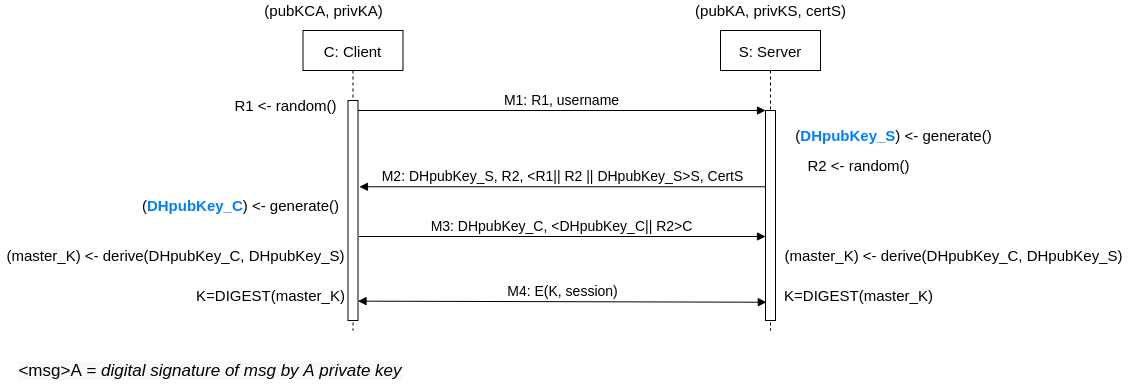
\includegraphics[scale=0.19]{img/AuthClientServer.png}
	\caption{Client Server Handshake Protocol Schema}
	\label {img: AuthClientServer}
\end{figure}
This handshake is a custom implementation of an ephimeral Diffie-Hellman Key Exchange, in which we ensure
protection against the man in the middle attack with random nuances (R1 and R2). The client is able to 
authenticate the server via it's certificate, signed by a trusted certification authority (the client
is distributed along with CA's self-signed certificate); the server have a built-in list of all client's
public keys. DH's private keys are deleted after the handshake and the key is generated by a digest of the 
shared seceret: in this way we provide security against a future disclousure of one of the long term private keys.

\newpage
\section{Chat Request}
With the client-server handshake we build a secure tunnel between each client and the server. Using this 
tunnel every client can execute command on the server in a secure way; the most important (and complex) command
is a chat request, of which we provide a scheme:
\begin{figure}[H]
	\centering
	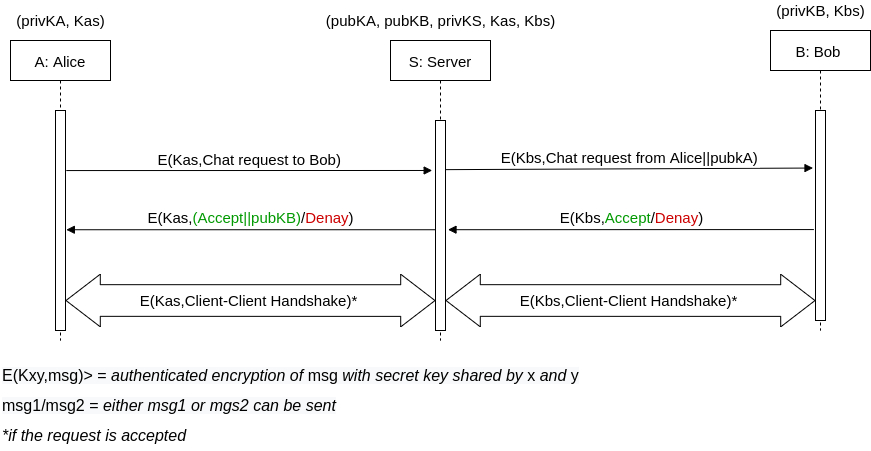
\includegraphics[scale=0.2]{img/ChatRequest.png}
	\caption{Chat Request Protocol Schema}
	\label {img: ChatRequest}
\end{figure}
The server is obliged to communicate correct public keys.
\section{Client to Client handshake}
In order to guarantee a secure communication of the clients agaist the server, we perform an ephimeral 
Diffie-Hellman Key Exchange befor starting the chat. In this case the two parties already know each other
public keys, because the server provided them. 
\begin{figure}[H]
	\centering
	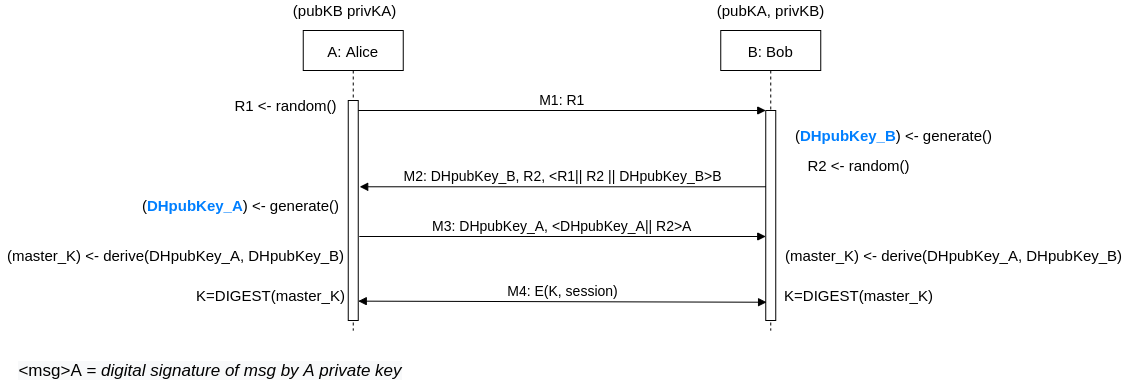
\includegraphics[scale=0.19]{img/AuthClientClient.png}
	\caption{Client Client Handshake Protocol Schema}
	\label {img: AuthClientClient}
\end{figure}
The server in not represented because it only retransmit messages from a client to the other without changing
anything; if the server try to implement a "man in the middle" attack he will only obtain a denial of service
because the protocol is protected by private key signatures. Also in this case, DH keys are discared after 
the handshake, and future messages are numbered againts reply attacks.

\section{Alghoritms and Protocols}
We briefly describe the cypher suite we choose to use in order to guarantee security specifications.
\subsection{Public Key Authentication}
\paragraph*{Long Term Keys}
The Cerification Authority (CA) have a \texttt{Publick Key}, included in a self-signed
certificate; the corresponding private key is embedded in the program for certificate generation, 
SimpleAuthority \footnote{https://simpleauthority.com}.
CA's cerficiate and Revocation List (CRL) are exported and distributed with client executable.
The server cerfificate, which is signed by CA, contains the \texttt{Publick Key} of the server; it
is stored server side, and provided to the client during the handshake.
Clients Public Keys are also stored in the server, while only the client hold its Private Key.
All keys are \texttt{RSA Key Pairs with 2048-bits Public Keys} and are stored in \texttt{.pem} format, as certificates and CRLs are.
\paragraph*{Short Term Keys}
Handshakes protocols are performed with the Ephimeral Diffie-Hellman Key Exchange. 
We choose to use the Elliptic Curve implenetation because is very efficent (in term of performance vs security strenght);
we use \verb|NID_X9_62_prime256v1| standard parameters that ensure 128-bits secuiry strenght with a 256-bits curve. We use the \texttt{SHA-256} digest of the \texttt{shared secret} as
the session key.
To ensure freshness in the challenge-response scheme we use \texttt{16 bytes nonces}.
\subsection{Authenticated Encryption}
From the handshake we obtain a 256-bits simmetric key which is used in \texttt{AES-256 GCM} authenticated encryprion protocol.
We use a \texttt{16 bytes} tag for authentication of cyphertext and clear fields in the header. GCM scheme ensure a cyphertext
size equal to the plaintext size; this makes programming easier, mantaining an optimal resistance against all known attacks.
Messages excanged in sessions are numbered, starting from 1, to a maximum of $2^{32}-1$ (\verb|0xFFFFFFFF|), which is the
maximum integer representable on 32 bits; this will make possible to identify a message reply, done
my an attacker. The session is automatically closed when a message with number \verb|0xFFFFFFFF| is recived.
Clients mantains two counter for the communication with the server:  one for the next message to send and another for
the next message to receive; the same thing is done for the communication with another client (to prevent the server to 
reply a message); also the server has to implement this behaveour in sessions with clients.
\chapter{Messages Format}

\section{Handshake}
\subsection*{Client Server Handshake}
\begin{figure}[H]
	\centering
	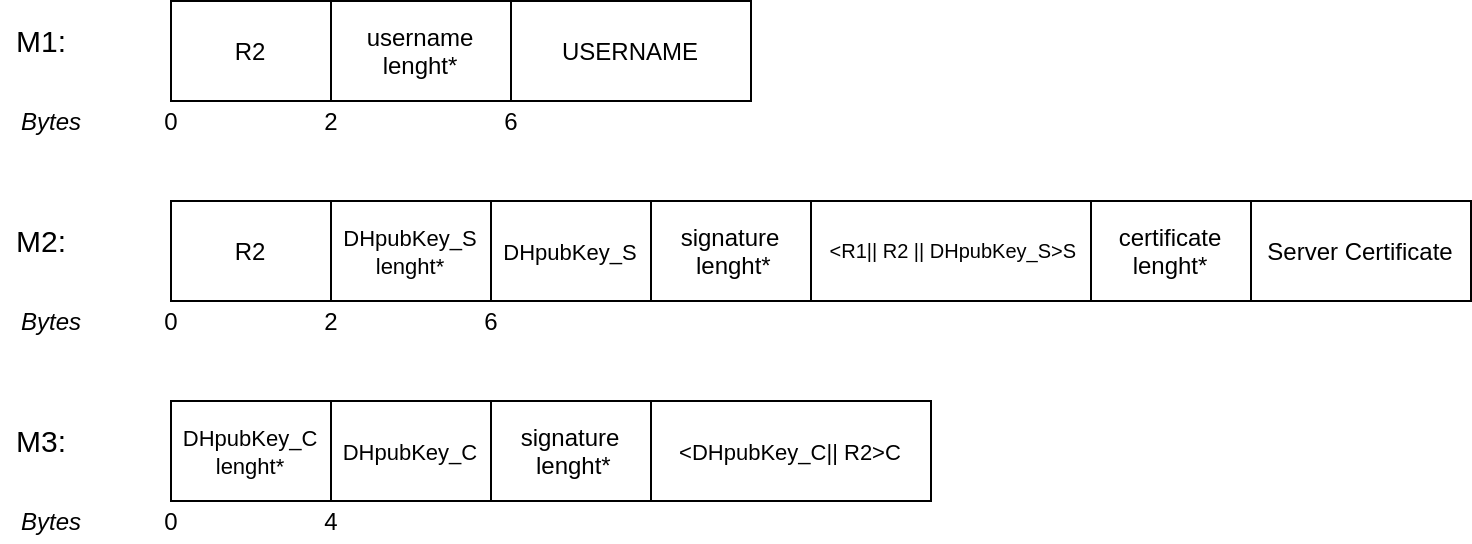
\includegraphics[scale=0.19]{img/AuthClientServer_messageFormat.png}
	\caption{Client Server Handshake Message Format}
	\label {img: FormatClientServer}
\end{figure}
\subsection*{Client Client Handshake}
\begin{figure}[H]
	\centering
	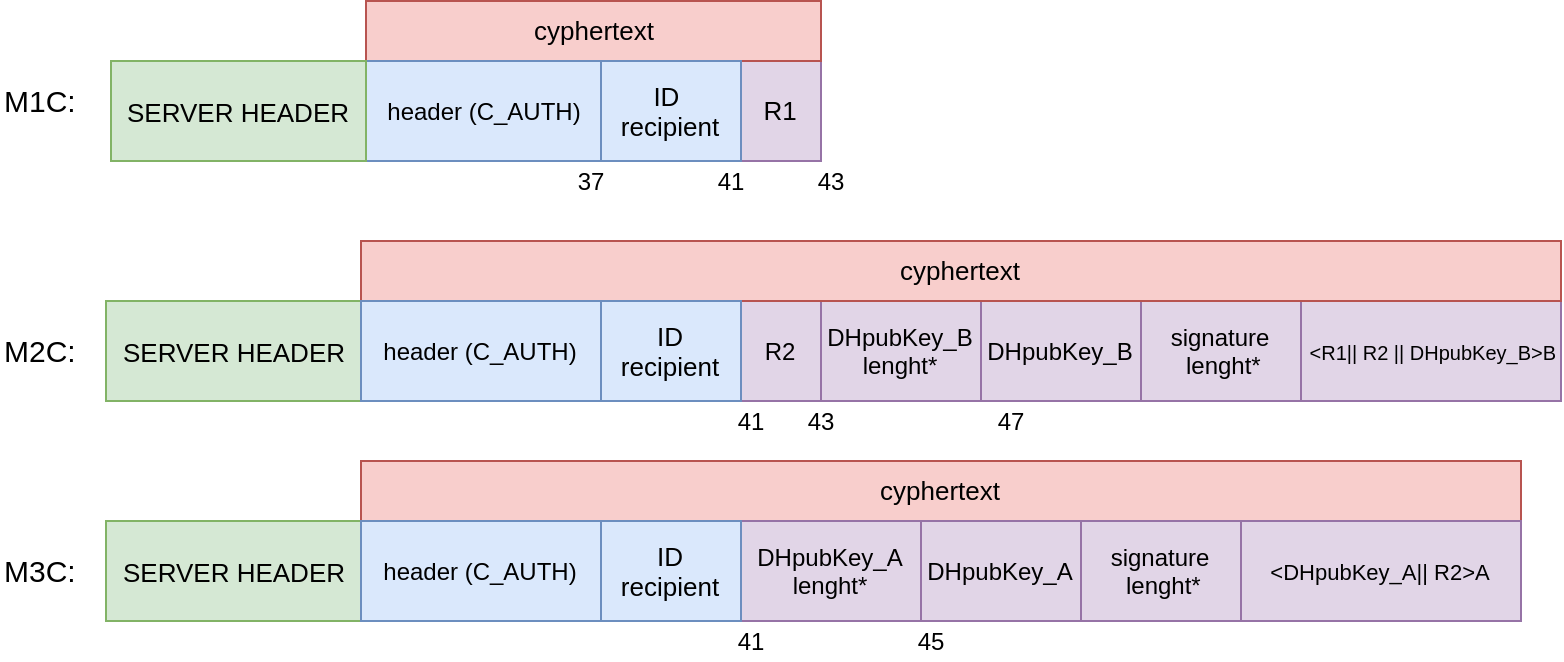
\includegraphics[scale=0.22]{img/AuthClientClient_messageFormat.png}
	\caption{Client Client Handshake Message Format}
	\label {img: FormatClientClient}
\end{figure}
\newpage
\section{Commands}
\subsection*{Client Online List Request and Answer }
\begin{figure}[H]
	\centering
	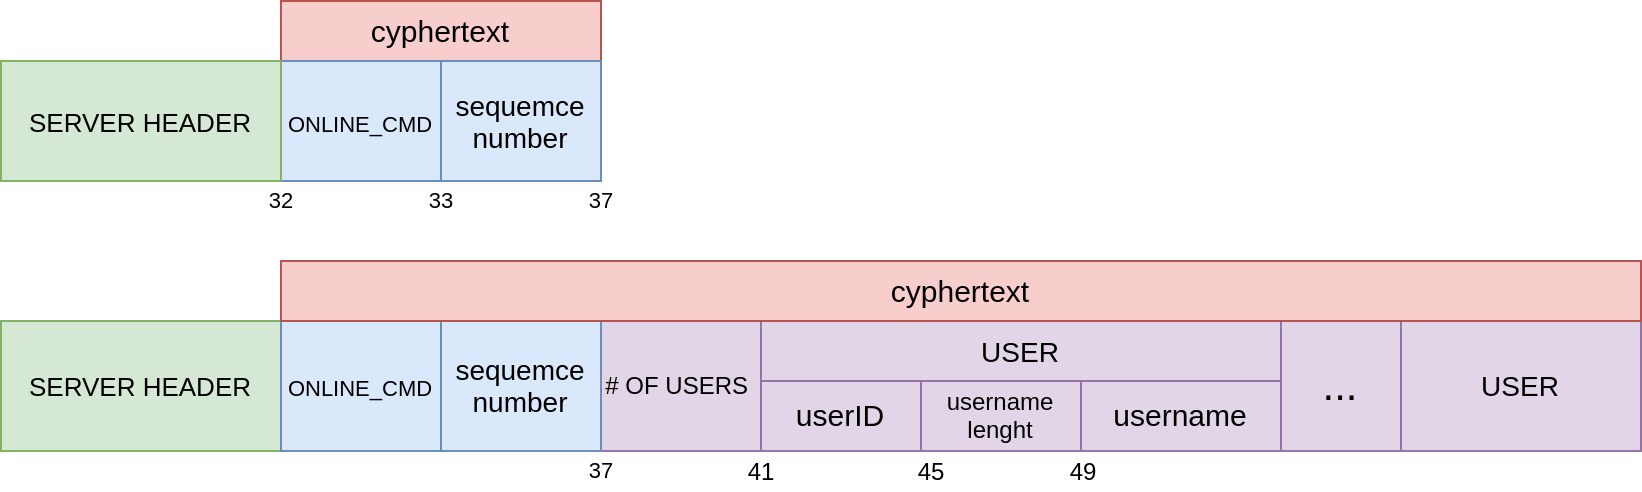
\includegraphics[scale=0.25]{img/ClientOnline_messageFormat.png}
	\caption{Client Online Message Format}
	\label {img: FormatClientOnline}
\end{figure}

\subsection*{Chat Request and Answers}
\begin{figure}[H]
	\centering
	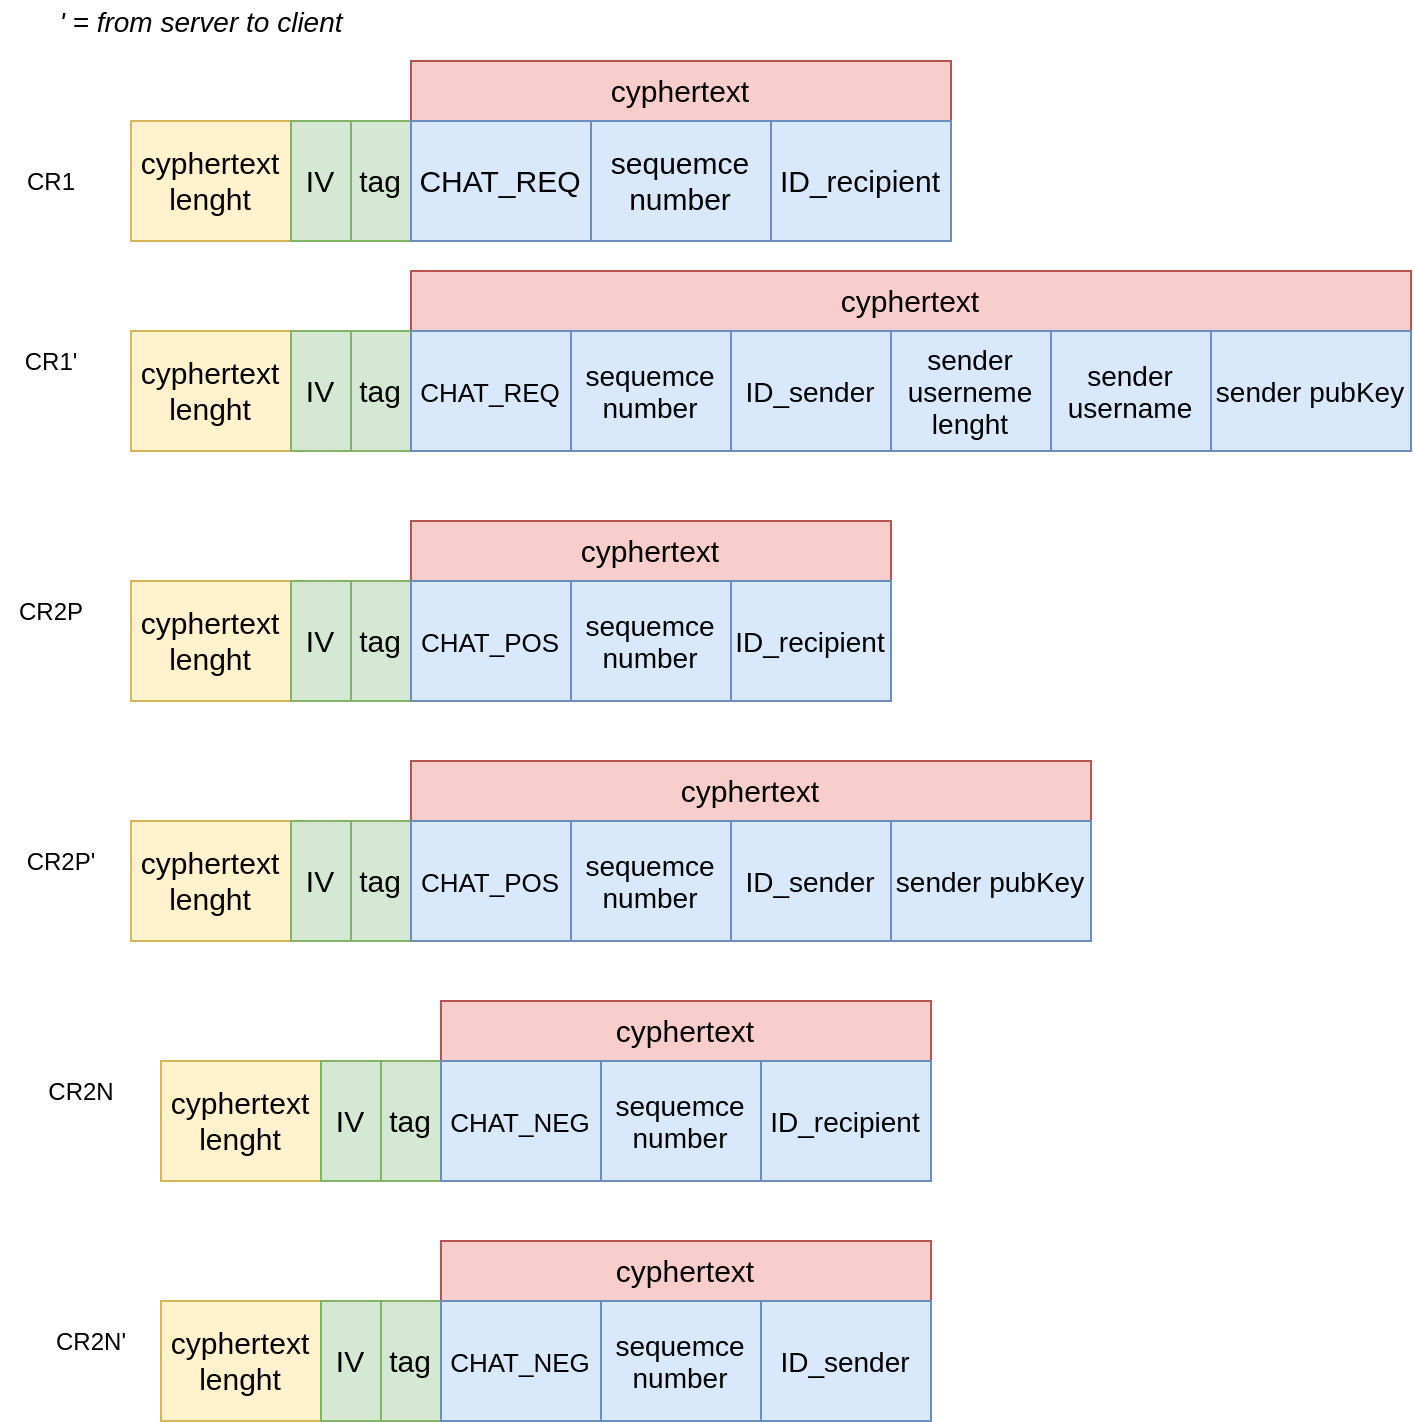
\includegraphics[scale=0.28]{img/ChatRequest_messageFormat.png}
	\caption{Chat Request Message Format}
	\label {img: FormatChatRequest}
\end{figure}
\newpage

\section{Chat}
\begin{figure}[H]
	\centering
	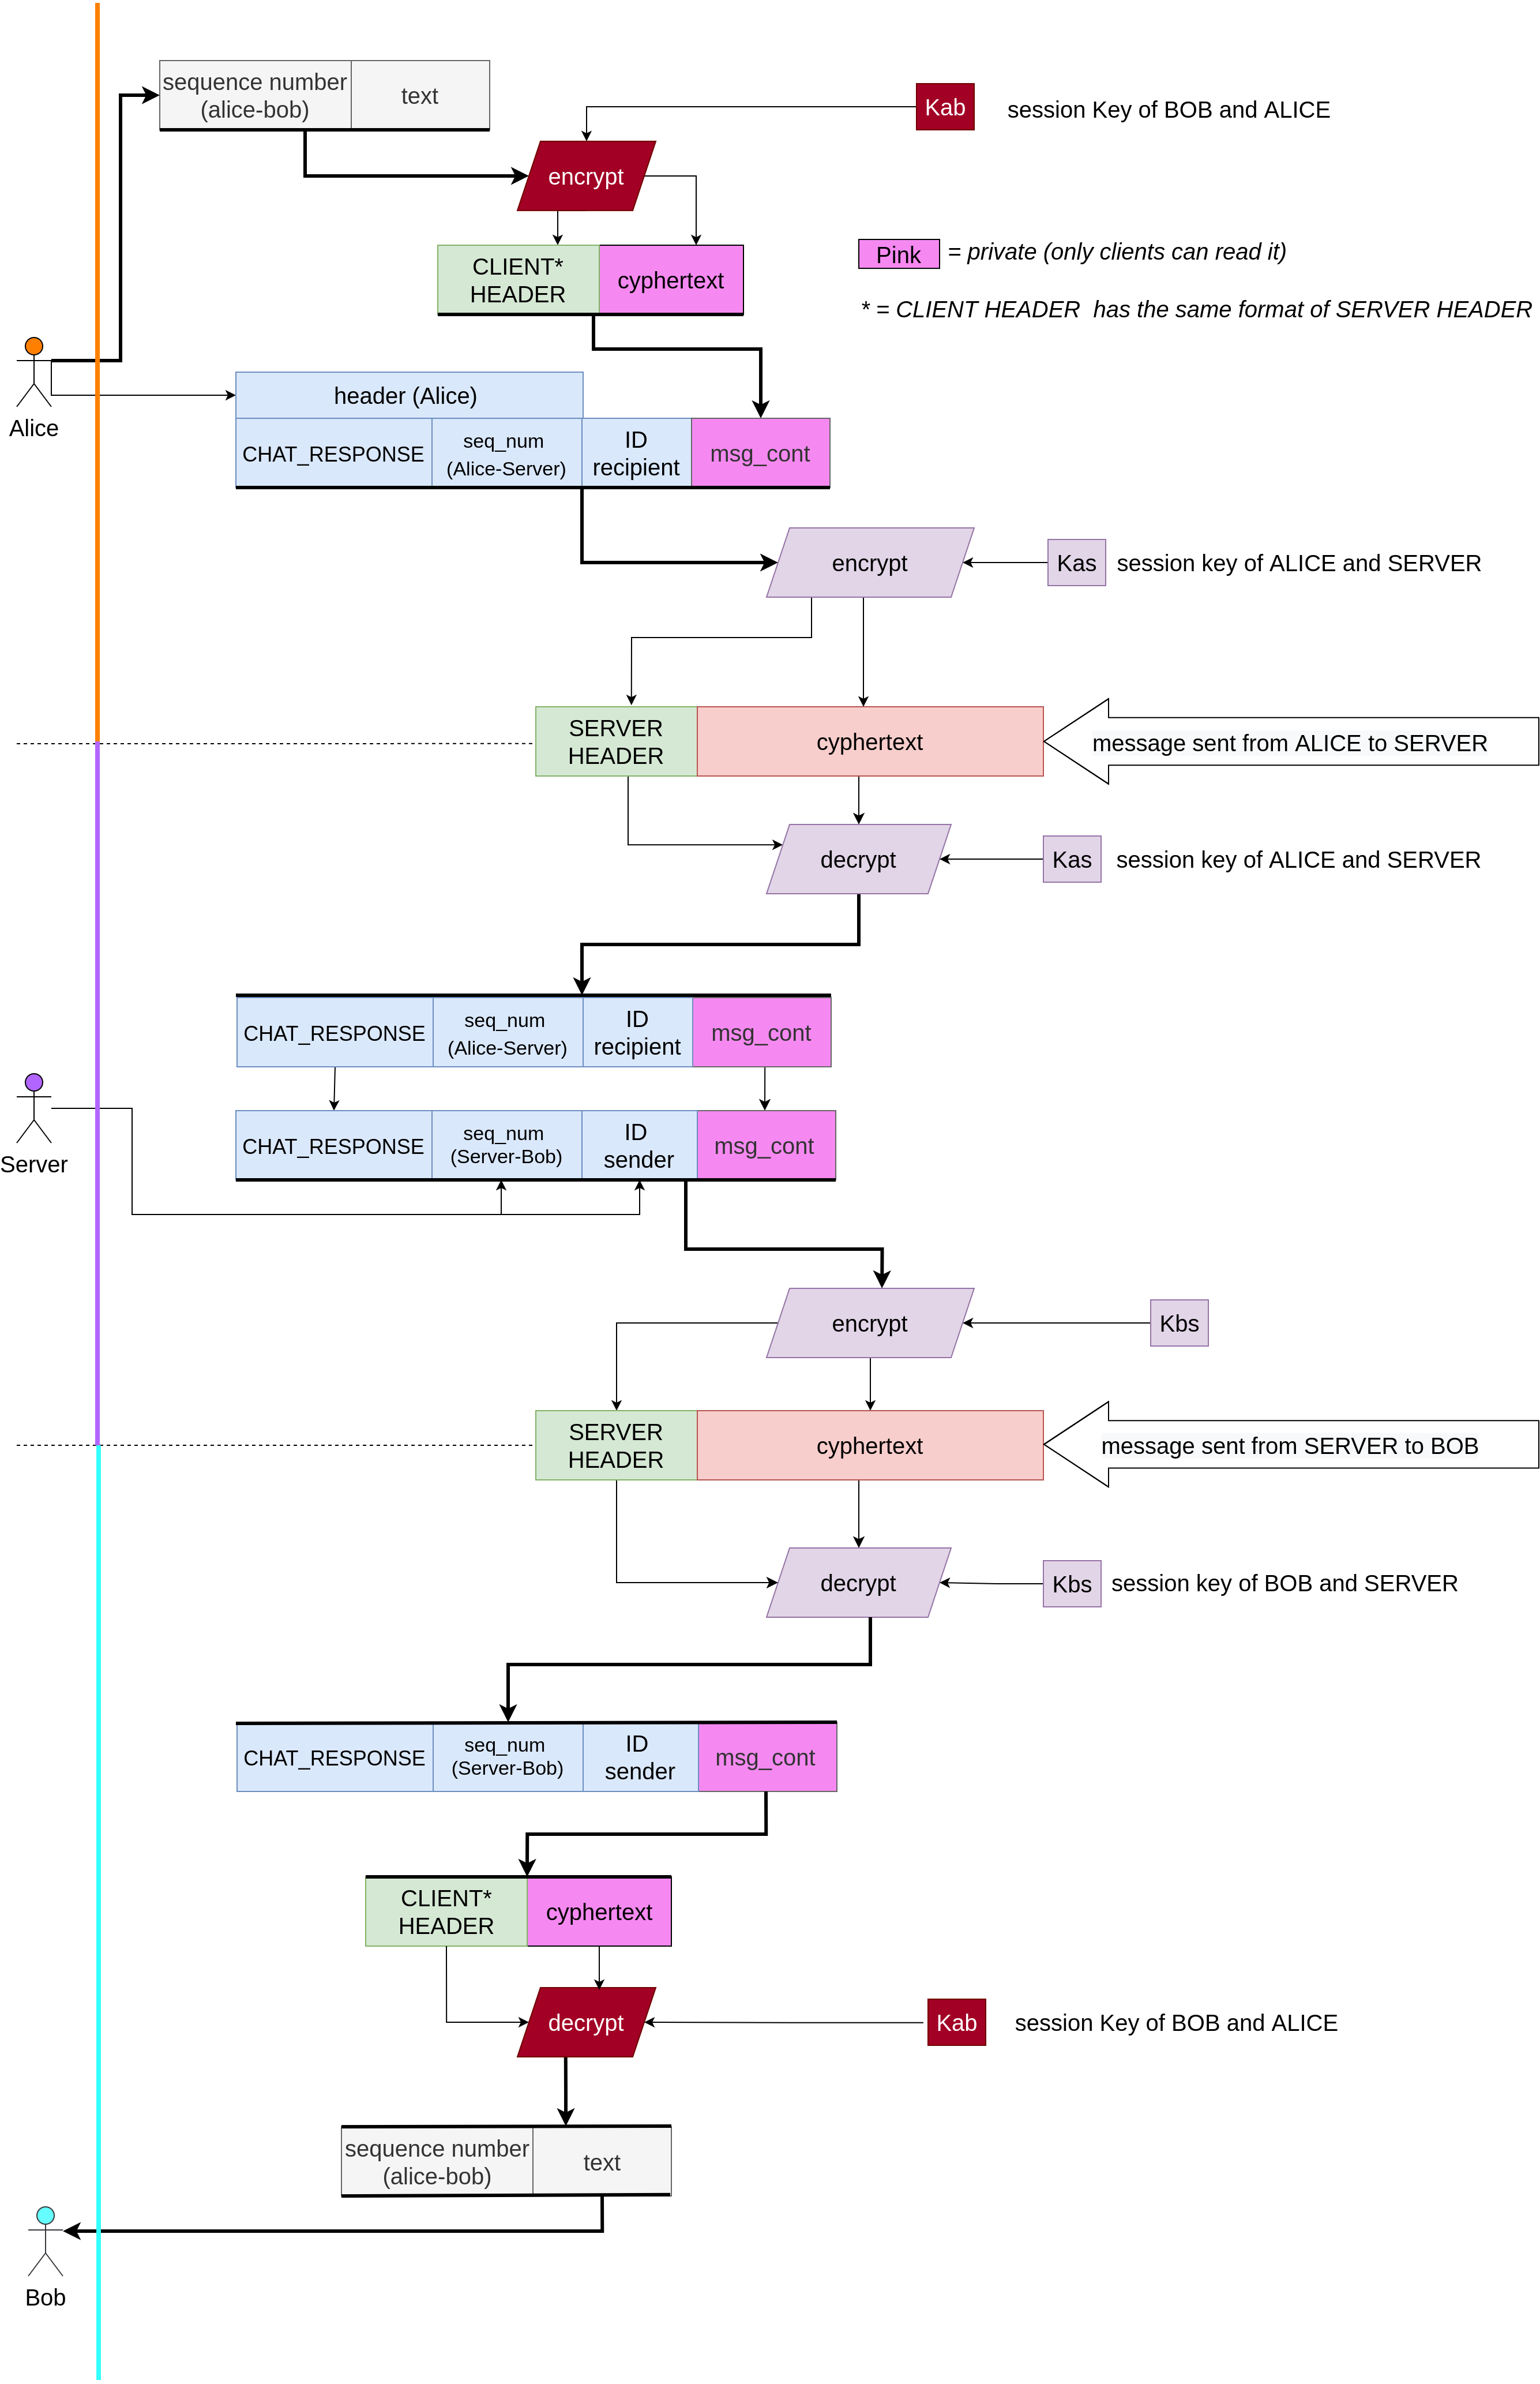
\includegraphics[scale=0.09]{img/message_relay.png}
	\caption{Client Client Handshake Protocol Schema}
	\label {img: MessageRelay}
\end{figure}

\section{How To Handle The Chat Request}
\noindent Let's start from the simple case in which a client wants to chat with another client and makes a request to the server: 
\begin{itemize}
	\item The standard channel is used to send either the request for chat and for the server's answers.
	\item If the target client accepts then the main process receive the confirmation from the server, then the main process set isChatting to true and it starts to chat.
\end{itemize}

\noindent When the server receive the command to chat with someone he has to send the chat request to the given client. Let suppose that Alice wants to chat with Bob. In this case the following steps must be performed:

\begin{itemize}
	\item The request must be done through the request channel
	\item The client daemon process (Alice's daemon process) is listening on its socket (see after) and receive the request, then it reads the variable isChatting: if it is true the daemon process refuses automatically the server request, otherwise it ask (HANDSHAKE) to the main process if he wants to speak with Bob. 
	\item The main process answer to the server by means of the daemon tools, if the answer is positive then it sets isChatting to true and so it waits for the message from Bob.
\end{itemize}

\noindent It's important to underline some concepts, first of all on the server side we have one process that handles two socket with the client, one for each channel. The protocol starts with the client that contacts the server, then the server and the client main process establish a connection and starts the protocol to establish a secure communication (Key Exchange). For standard messages this standard channel is used.

\begin{figure}[H]
	\centering
	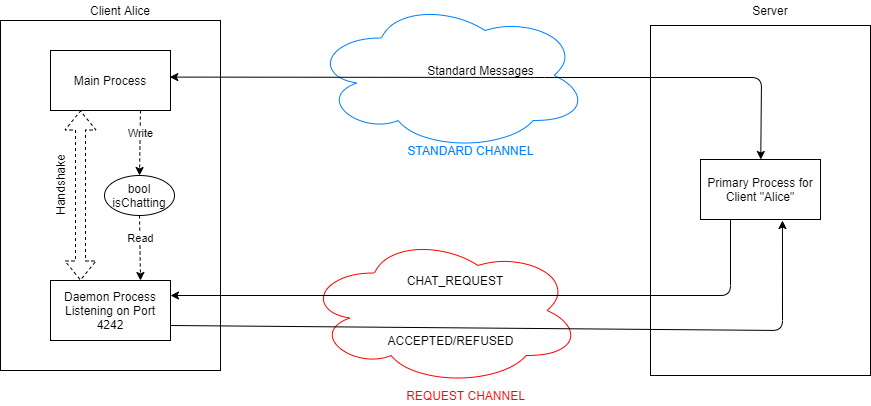
\includegraphics[scale=0.2]{img/chatRequestProtocolOneProcess.png}
	\caption{Protocol Schema}
	\label {img: chatRequestProtocolOneProcess}
\end{figure}

\noindent When the server has to sent a chat request to this client the request channel must be used. Thus it establishes a connection with the daemon process of the client that works as a server process and it is listening on port 4242 (see figure \ref{img: chatRequestProtocolOneProcess}). The security of this secondary channel is ensured by the fact that the messages sent by the server to the client on the request channel are encrypted with the shared key established during the handshake in the standard channel, hence we can say that the authentication problem is not present. In any case to implement a greater security is possible to generate client side a one time password that is sent to the server in the encrypted session through the standard channel, then the server will sent this otp to the client daemon process to identify itself.
	

\noindent Other things to take in mind are:
\begin{itemize}
	\item We assume that who send the chat request is the first to send messages.
	\item On the server side for each client two socket must be established, one for the standard channel and another one for the request channel but the process for each client is only one.
\end{itemize}



	
%	\item A third solution can be adding a command to indicate that a client is available to receive chat request. Thus:
	
%	\begin{enumerate}
%		\item A users is online when it has launched the command "available" (isChatting = false). Notice that in this case the variable isChatting can be called in a more correct way isAvailable.
		
%		\item  A users is offline (isChatting = false) if it is not available (if he has not launched the command available or if he is chatting with someone else). In that case offline means also busy whereas online means also available.
%	\end{enumerate}

	
%\end{enumerate}

%here are two possibilities:
%\begin{enumerate}
%	\item Two processes, one for the client main process and another one for the client daemon process. See figure \ref{img: chatRequestProtocolTwoProcesses}.
	
%	\begin{figure}[htpb]
%		\centering
%		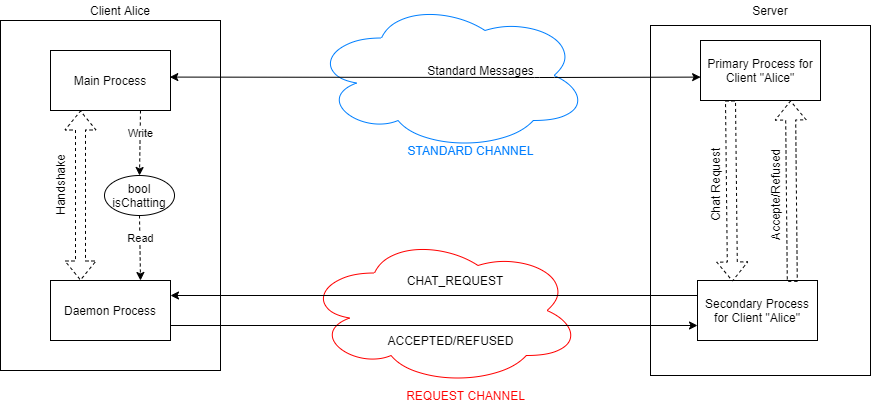
\includegraphics[scale=0.5]{img/chatRequestProtocolTwoProcesses.png}
%		\caption{Solution with two processes}
%		\label {img: chatRequestProtocolTwoProcesses}
%	\end{figure}

%\noindent Notes:


\end{document}          
